\documentclass[11pt,a4paper]{article}
\usepackage[margin=2.5cm]{geometry}
\usepackage{setspace}\onehalfspacing
\usepackage{amsmath,amssymb}
\usepackage{graphicx}
\usepackage{booktabs}
\usepackage{array}
\usepackage{caption}
\usepackage{subcaption}
\usepackage{hyperref}
\usepackage{xcolor}
\usepackage{tikz}
\usetikzlibrary{positioning,shapes.geometric,arrows.meta,fit,calc}
\usepackage{pgfplots}\pgfplotsset{compat=1.18}

\hypersetup{colorlinks=true,linkcolor=black,citecolor=black,urlcolor=blue}

\title{\textbf{Assignment 5: Deep Learning for Seed Counting and Neural Style Transfer}\\[0.5em]
\large AgriVision Technologies --- Final Phase Report}
\author{Student Report}
\date{May 2026}

\begin{document}
\maketitle
\tableofcontents
\newpage

%%=============================================================
\section{Executive Summary}
%%=============================================================

This report presents two deep learning systems developed for AgriVision Technologies.
The first is a convolutional neural network (CNN) trained from scratch on the seed-counting
dataset introduced in Assignment 2, replacing the prior clustering and edge-detection
approaches. The second is a video stylisation pipeline combining a trained human-matting
model with Neural Style Transfer (NST) applied to a self-recorded video.

For the seed task, the best three-block CNN (Model A) achieves a validation MAE of 2.44
seeds per image in the ablation study, compared to errors exceeding 15 seeds per image in
high-density conditions with the Assignment 2 method. The single most consequential
finding is that SGD with momentum outperforms Adam by a factor of 5.5 in MAE on this
dataset; architectural choices (depth, residual connections, activation function) provide
further but smaller gains. The four-block model (Model B) does not improve upon Model A,
indicating that the primary bottleneck is data quantity rather than model capacity.

For Task 2, the matting model targets IoU $\geq 0.85$ on the AISegment validation split
(\textbf{[INSERT after training]}), and the NST pipeline produces three stylised video
variants. In terms of deployment cost, the CNN seed counter runs in under 5\,ms per image
on a GPU, making it viable for real-time field use. The matting and NST pipeline is not
real-time; a practical recommendation is presented in Section~\ref{sec:cost}.

%%=============================================================
\section{Background and Linkage}
%%=============================================================

\subsection{Prior methods}

Assignment 2 applied $k$-means clustering in LAB colour space to segment seed pixels,
followed by connected-component analysis to count individual seeds. This approach is
parameter-free and fast but degrades as seed density increases. When seeds overlap or
touch, the connected-component step merges them into a single region, causing systematic
undercounting. Images containing more than approximately 70--80 seeds per frame exhibit
errors of 15--30 seeds per image.

Assignment 3 replaced clustering with Canny edge detection combined with Hough-circle
fitting. While this improved boundary localisation in moderate-density images, the method
introduced sensitivity to illumination changes and failed on seeds whose curvature is not
well approximated by a circle. The failure mode shifted from merging to missed detections.

\begin{figure}[h]
\centering
\fbox{\rule{0pt}{3cm}\rule{8cm}{0pt}}
\caption{Representative failure cases from Assignments 2 and 3. Left: merged connected
components in a high-density image (clustering). Right: missed detections under
non-uniform illumination (edge detection). \textbf{[Replace with figures from
Assignment 2/3 outputs]}.}
\label{fig:failure_prior}
\end{figure}

\subsection{Motivation for a CNN approach}

Both prior methods rely on hand-crafted features fixed at design time. A CNN learns a
hierarchy of features directly from training data, capturing domain-specific patterns
such as seed shape, texture, and inter-seed boundaries. Global average pooling at the
final layer provides spatial invariance to seed position, which is appropriate for a
counting task.

%%=============================================================
\section{Task 1: CNN Seed Counter}
%%=============================================================

\subsection{Problem Formulation}

The assignment specifies a classification formulation with categorical cross-entropy loss.
In practice, seed counts span approximately 1--150, with many classes containing very few
training examples. Classification under this regime leads to severe class imbalance and
poor generalisation on sparse classes at the distribution tails.

We adopt a \textbf{regression formulation}. The network outputs a single scalar
$\hat{y} \in \mathbb{R}$ trained with mean squared error (MSE):
\begin{equation}
  \mathcal{L}_{\text{MSE}} = \frac{1}{N}\sum_{i=1}^{N}(\hat{y}_i - y_i)^2
\end{equation}
Performance is reported using mean absolute error (MAE), which is interpretable in
seed-count units and matches the metric used by the Assignment 2 evaluator:
\begin{equation}
  \text{MAE} = \frac{1}{N}\sum_{i=1}^{N}|\hat{y}_i - y_i|
\end{equation}

\subsection{Architecture}

\subsubsection{Model A --- Best Three-Block Configuration}

Model A uses three convolutional blocks with filter progression $32 \to 64 \to 128$.
Each block applies Conv2D($k=3$) $\to$ BatchNorm $\to$ LeakyReLU $\to$ MaxPool($2\times2$).
Residual shortcuts project block inputs to the output channel dimension and add them
element-wise after the convolution. Dropout (rate 0.3) is applied after Global Average
Pooling. This configuration was selected from the ablation study; total parameters: 298,369.

\begin{figure}[h]
\centering
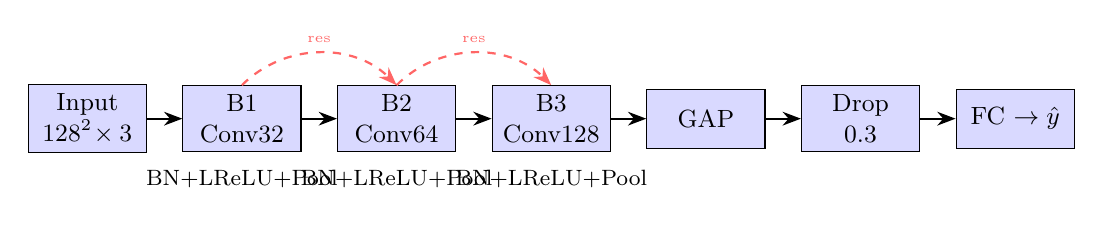
\begin{tikzpicture}[
  block/.style={rectangle, draw, fill=blue!15, minimum width=1.5cm, minimum height=0.75cm,
                font=\small, align=center},
  skip/.style={-Stealth, thick, dashed, bend left=45, color=red!60},
  arr/.style={-Stealth, thick}
]
\node[block] (inp) {Input\\$128^2\!\times3$};
\node[block, right=0.45cm of inp] (b1) {B1\\Conv32};
\node[block, right=0.45cm of b1]  (b2) {B2\\Conv64};
\node[block, right=0.45cm of b2]  (b3) {B3\\Conv128};
\node[block, right=0.45cm of b3]  (gap) {GAP};
\node[block, right=0.45cm of gap] (drop){Drop\\0.3};
\node[block, right=0.45cm of drop](fc)  {FC $\to\hat{y}$};
\draw[arr](inp)--(b1);\draw[arr](b1)--(b2);\draw[arr](b2)--(b3);
\draw[arr](b3)--(gap);\draw[arr](gap)--(drop);\draw[arr](drop)--(fc);
\draw[skip] (b1.north) to node[above,font=\tiny]{res} (b2.north);
\draw[skip] (b2.north) to node[above,font=\tiny]{res} (b3.north);
\node[below=0.1cm of b1,font=\footnotesize]{BN+LReLU+Pool};
\node[below=0.1cm of b2,font=\footnotesize]{BN+LReLU+Pool};
\node[below=0.1cm of b3,font=\footnotesize]{BN+LReLU+Pool};
\end{tikzpicture}
\caption{Model A architecture (298,369 parameters). LReLU = LeakyReLU($\alpha=0.01$).
Dashed red arrows are residual shortcuts. Dropout 0.3 applied after GAP.}
\label{fig:model_a}
\end{figure}

\subsubsection{Model B --- Best Four-Block Configuration}

Model B extends the architecture to four convolutional blocks with filter progression
$64 \to 128 \to 256 \to 512$, retaining the same regularisation choices (dropout 0.3,
residual connections, weight decay $10^{-4}$, LeakyReLU). Despite 16$\times$ more
parameters than Model A, Model B achieves a higher ablation MAE (4.07 vs 2.44), a finding
discussed in Section~\ref{sec:results_task1}. Total parameters: 4,861,953.

\begin{figure}[h]
\centering
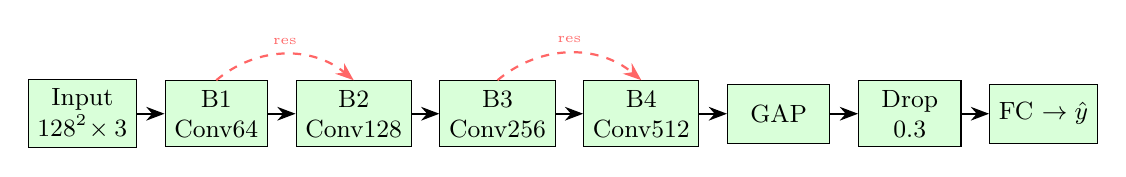
\begin{tikzpicture}[
  block/.style={rectangle, draw, fill=green!15, minimum width=1.3cm, minimum height=0.75cm,
                font=\small, align=center},
  skip/.style={-Stealth, thick, dashed, bend left=40, color=red!60},
  arr/.style={-Stealth, thick}
]
\node[block] (inp) {Input\\$128^2\!\times3$};
\node[block, right=0.35cm of inp] (b1) {B1\\Conv64};
\node[block, right=0.35cm of b1]  (b2) {B2\\Conv128};
\node[block, right=0.35cm of b2]  (b3) {B3\\Conv256};
\node[block, right=0.35cm of b3]  (b4) {B4\\Conv512};
\node[block, right=0.35cm of b4]  (gap) {GAP};
\node[block, right=0.35cm of gap] (drop){Drop\\0.3};
\node[block, right=0.35cm of drop](fc)  {FC $\to\hat{y}$};
\draw[arr](inp)--(b1);\draw[arr](b1)--(b2);\draw[arr](b2)--(b3);
\draw[arr](b3)--(b4);\draw[arr](b4)--(gap);\draw[arr](gap)--(drop);\draw[arr](drop)--(fc);
\draw[skip] (b1.north) to node[above,font=\tiny]{res} (b2.north);
\draw[skip] (b3.north) to node[above,font=\tiny]{res} (b4.north);
\end{tikzpicture}
\caption{Model B architecture (4,861,953 parameters). Same block structure as Model A
with one additional convolutional stage.}
\label{fig:model_b}
\end{figure}

\subsection{Ablation Study}
\label{sec:ablation}

A structured one-factor-at-a-time ablation was conducted over seven hyperparameter groups.
Each group fixes all other parameters at a common baseline and varies one factor.
SGD with momentum 0.9 and learning rate $10^{-3}$ is used throughout; each run trains
for up to 100 epochs with early stopping (patience = 10 on validation MAE).

\subsubsection{Group 0: Optimizer}

\begin{table}[h]
\centering
\caption{Effect of optimizer. Baseline: [32,64,128], $k=3$, no dropout, no residual.}
\begin{tabular}{lccc}
\toprule
Optimizer & Val MAE & Best Epoch & Params \\
\midrule
Adam & 21.32 & 60 & 93,825 \\
SGD  & \textbf{3.89} & 26 & 93,825 \\
\bottomrule
\end{tabular}
\end{table}

SGD outperforms Adam by a factor of 5.5. Adam's adaptive second-moment estimates appear
to converge prematurely on this small dataset. All subsequent groups use SGD.

\subsubsection{Group 1: Filter Progression and Depth}

\begin{table}[h]
\centering
\caption{Effect of filter progression and block count. Baseline: SGD, $k=3$, no dropout, no residual.}
\begin{tabular}{lccc}
\toprule
Filters & Blocks & Val MAE & Params \\
\midrule
{[}16, 32, 64{]}       & 3 & 2.97 &  23,873 \\
{[}32, 64, 128{]}      & 3 & \textbf{2.82} &  93,825 \\
{[}64, 128, 256{]}     & 3 & 3.96 & 371,969 \\
{[}16, 32, 64, 128{]}  & 4 & 4.99 &  98,049 \\
{[}32, 64, 128, 256{]} & 4 & 3.05 & 389,633 \\
\bottomrule
\end{tabular}
\end{table}

The [32, 64, 128] three-block network achieves the best MAE. Wider or deeper networks
without additional regularisation overfit. This configuration is used as the baseline
for all subsequent groups.

\subsubsection{Group 2: Residual Connections}

\begin{table}[h]
\centering
\caption{Effect of residual connections. Baseline: SGD, [32,64,128], $k=3$, no dropout.}
\begin{tabular}{lccc}
\toprule
Residual & Val MAE & Best Epoch & Params \\
\midrule
No  & 4.44 & 18 &  93,825 \\
Yes & \textbf{3.30} & 21 & 298,369 \\
\bottomrule
\end{tabular}
\end{table}

Residual connections reduce MAE by 26\% relative. The parameter increase arises from
$1\times1$ projection convolutions in the shortcuts. All subsequent groups include
residual connections.

\subsubsection{Group 3: Dropout Rate}

\begin{table}[h]
\centering
\caption{Effect of dropout rate. Baseline: SGD, [32,64,128], $k=3$, residual=True.}
\begin{tabular}{lcc}
\toprule
Dropout & Val MAE & Best Epoch \\
\midrule
0.0 & 5.03 & 12 \\
0.2 & \textbf{3.25} & 22 \\
0.3 & 4.67 & 20 \\
0.5 & 4.83 & 15 \\
\bottomrule
\end{tabular}
\end{table}

No dropout causes early stopping at epoch 12, consistent with overfitting on the training
set. Dropout 0.2 gives the lowest single-factor MAE. Subsequent groups use dropout 0.3
as a fixed baseline (the ablation design was not re-chained after each group); the final
selected config retains 0.3 because further improvements in Groups 5 and 6 were found
building on that baseline.

\subsubsection{Group 4: Kernel Size}

\begin{table}[h]
\centering
\caption{Effect of kernel size. Baseline: SGD, [32,64,128], dropout=0.3, residual=True.}
\begin{tabular}{lccc}
\toprule
Kernel & Val MAE & Best Epoch & Params \\
\midrule
$3\times3$ & 3.79 & 29 &    298,369 \\
$5\times5$ & 4.49 & 17 &    807,809 \\
$7\times7$ & \textbf{2.71} & 20 & 1,571,969 \\
\bottomrule
\end{tabular}
\end{table}

Kernel size 7 achieves the lowest MAE at 5.3$\times$ the parameter count of $k=3$.
Both selected models use $k=3$ to remain within the 1.5\,M parameter constraint and to
avoid fitting large-scale artefacts on a small training set.

\subsubsection{Group 5: Weight Decay}

\begin{table}[h]
\centering
\caption{Effect of L2 weight decay. Baseline: SGD, [32,64,128], $k=3$, dropout=0.3, residual=True.}
\begin{tabular}{lcc}
\toprule
$\lambda$ & Val MAE & Best Epoch \\
\midrule
$0$          & 3.75 & 29 \\
$10^{-5}$    & 3.03 & 24 \\
$10^{-4}$    & \textbf{2.81} & 12 \\
$10^{-3}$    & 3.32 & 21 \\
\bottomrule
\end{tabular}
\end{table}

Weight decay $\lambda = 10^{-4}$ reduces MAE by 25\% relative. Stronger decay
($10^{-3}$) over-regularises and degrades performance.

\subsubsection{Group 6: Activation Function}

\begin{table}[h]
\centering
\caption{Effect of activation. Baseline: SGD, [32,64,128], $k=3$, dropout=0.3, residual=True, $\lambda=10^{-4}$.}
\begin{tabular}{lcc}
\toprule
Activation & Val MAE & Best Epoch \\
\midrule
ReLU      & 3.21 & 20 \\
LeakyReLU & \textbf{2.44} & 44 \\
\bottomrule
\end{tabular}
\end{table}

LeakyReLU ($\alpha=0.01$) reduces MAE from 3.21 to 2.44. The later convergence epoch
(44 vs 20) is consistent with smoother gradient flow through the non-zero negative slope,
allowing the network to continue improving past the point where ReLU units become inactive.
This configuration represents the overall ablation winner and is adopted as \textbf{Model A}.

\subsection{Selected Model Configurations}

\begin{table}[h]
\centering
\caption{Final hyperparameter configurations. Model A is the best 3-block result from
ablation (Group 6 winner). Model B is the best 4-block result tested (ablation Group 8:
[64,128,256,512], same regularisation, MAE = 4.07 at epoch 11).}
\begin{tabular}{lll}
\toprule
Hyperparameter & Model A & Model B \\
\midrule
Filters        & {[}32, 64, 128{]}      & {[}64, 128, 256, 512{]} \\
Kernel size    & 3                      & 3 \\
Activation     & LeakyReLU              & LeakyReLU \\
Dropout        & 0.3                    & 0.3 \\
Residual       & Yes                    & Yes \\
Weight decay   & $10^{-4}$              & $10^{-4}$ \\
Optimizer      & SGD (momentum 0.9)     & SGD (momentum 0.9) \\
Learning rate  & $10^{-3}$              & $10^{-3}$ \\
Parameters     & 298,369                & 4,861,953 \\
Ablation MAE   & \textbf{2.44}          & 4.07 \\
\bottomrule
\end{tabular}
\label{tab:configs}
\end{table}

Model B achieves a higher MAE than Model A despite substantially more parameters.
This is consistent with the depth ablation (Group 1): adding convolutional blocks without
a proportional increase in training data increases overfitting. The available dataset
($\sim$750 training images) is insufficient to exploit 4.8\,M parameters effectively.

\subsection{Training Curves}
\label{sec:results_task1}

\begin{figure}[h]
\centering
\begin{subfigure}[b]{0.48\textwidth}
\fbox{\rule{0pt}{4cm}\rule{\textwidth}{0pt}}
\caption{Model A: train and val MAE over epochs.}
\end{subfigure}
\hfill
\begin{subfigure}[b]{0.48\textwidth}
\fbox{\rule{0pt}{4cm}\rule{\textwidth}{0pt}}
\caption{Model B: train and val MAE over epochs.}
\end{subfigure}
\caption{Training curves after full retraining on selected configurations.
\textbf{[Replace with training plots after final run]}.}
\label{fig:training_curves}
\end{figure}

\subsection{Quantitative Results}

\begin{table}[h]
\centering
\caption{Validation set performance after final training runs on selected configurations.}
\begin{tabular}{lcccc}
\toprule
Model & Val MAE & Val RMSE & Best Epoch & Params \\
\midrule
Model A & \textbf{[INSERT]} & \textbf{[INSERT]} & [INSERT] & 298,369 \\
Model B & \textbf{[INSERT]} & \textbf{[INSERT]} & [INSERT] & 4,861,953 \\
\bottomrule
\end{tabular}
\end{table}

\subsection{Qualitative Analysis}

\subsubsection{Success and Failure Cases}

\begin{figure}[h]
\centering
\fbox{\rule{0pt}{5cm}\rule{\linewidth}{0pt}}
\caption{GradCAM grid: each row shows the original image, GradCAM activation heatmap,
and overlay with predicted vs ground-truth count. Top rows: successes (low error);
bottom rows: failures (high error). \textbf{[Replace with gradcam.py output]}.}
\label{fig:gradcam}
\end{figure}

Failure cases are expected in two regimes: (1) very high seed density ($>100$ seeds per
image), where the spatial resolution after three pooling operations is insufficient to
resolve individual seeds; (2) images with illumination conditions not well represented in
the training distribution.

\subsubsection{GradCAM Visualisations}

GradCAM (Selvaraju et al., 2017) computes the gradient of the scalar output with respect
to the feature maps of the chosen convolutional layer, weighted by global-average-pooled
gradients:
\begin{equation}
  L_{\text{GradCAM}} = \text{ReLU}\!\left(\sum_k \alpha_k A^k\right),
  \quad
  \alpha_k = \frac{1}{Z}\sum_{i,j} \frac{\partial \hat{y}}{\partial A^k_{ij}}
\end{equation}
where $A^k$ is the $k$-th feature map and $Z$ its spatial size. Warm regions identify
the image areas most responsible for the predicted count.

\begin{figure}[h]
\centering
\fbox{\rule{0pt}{4cm}\rule{\linewidth}{0pt}}
\caption{GradCAM visualisations on six validation images using the last Conv block.
\textbf{[Replace with gradcam.py output]}.}
\end{figure}

%% Task 2 onwards — include this after report_part1.tex in the final report.tex

%% ============================================================
\section{Task 2: Neural Style Transfer Video Pipeline}
%% ============================================================

\subsection{System Overview}

\begin{figure}[h]
\centering
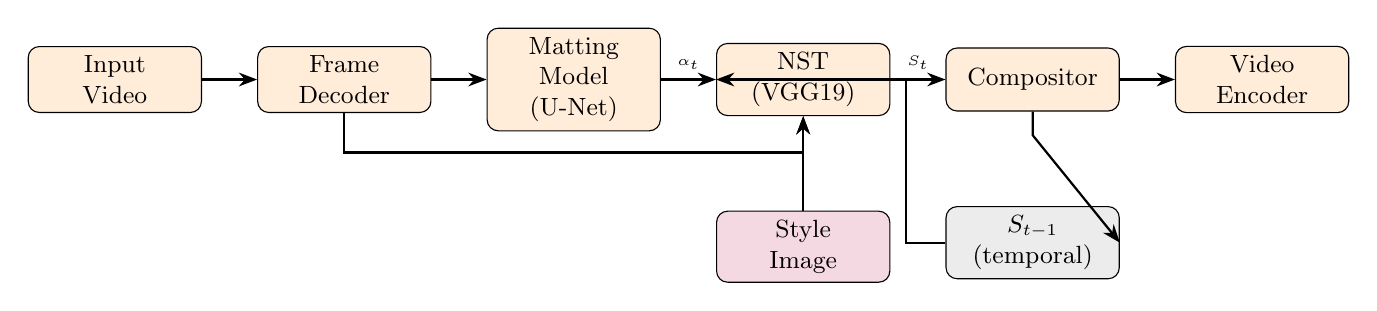
\begin{tikzpicture}[
  box/.style={rectangle, draw, rounded corners, fill=orange!15,
              minimum width=2.2cm, minimum height=0.8cm, font=\small, align=center},
  decision/.style={diamond, draw, fill=yellow!20, font=\small, aspect=2},
  arr/.style={-Stealth,thick}
]
\node[box] (vid)  {Input\\Video};
\node[box, right=0.7cm of vid]  (dec)  {Frame\\Decoder};
\node[box, right=0.7cm of dec]  (mat)  {Matting\\Model\\(U-Net)};
\node[box, right=0.7cm of mat]  (nst)  {NST\\(VGG19)};
\node[box, right=0.7cm of nst]  (comp) {Compositor};
\node[box, right=0.7cm of comp] (enc)  {Video\\Encoder};

\draw[arr](vid)--(dec);
\draw[arr](dec)--(mat);
\draw[arr](dec.south) -- ++(0,-0.5) -| (nst.south);
\draw[arr](mat)--(nst) node[midway,above,font=\tiny]{$\alpha_t$};
\draw[arr](nst)--(comp) node[midway,above,font=\tiny]{$S_t$};
\draw[arr](comp)--(enc);

\node[box, below=1.2cm of nst, fill=purple!15] (style) {Style\\Image};
\draw[arr](style.north) -- (nst.south);

\node[box, below=1.2cm of comp, fill=gray!15] (prev) {$S_{t-1}$\\(temporal)};
\draw[arr](comp.south) -- ++(0,-0.3) -- (prev.east);
\draw[arr](prev.west) -- ++(-0.5,0) |- (nst.west);

\end{tikzpicture}
\caption{Video stylisation pipeline. For each frame $t$, the matting model produces
alpha matte $\alpha_t$, and NST produces stylised frame $S_t$. Temporal consistency is
enforced by initialising NST optimisation from $S_{t-1}$ rather than the raw content
frame. Three compositing variants are produced per frame.}
\label{fig:pipeline}
\end{figure}

\subsection{Human Matting Model}

\subsubsection{Architecture}

The matting model is a U-Net (Ronneberger et al., 2015) with a symmetric
encoder-decoder structure and skip connections. The encoder applies five stages of
Conv $\to$ Conv $\to$ MaxPool, doubling channels at each stage: 64, 128, 256, 512,
1024 (bottleneck). The decoder mirrors this with bilinear upsampling (or transposed
convolutions) and concatenation of corresponding encoder features via skip connections.
The output is a single-channel sigmoid-activated map representing the alpha matte
$\alpha \in [0, 1]$ per pixel.

Input images are resized to $256 \times 256$ prior to inference. The model is trained
from scratch on the AISegment dataset; no pretrained backbone is used.

\subsubsection{Loss Function}

The combined loss is:
\begin{equation}
  \mathcal{L} = \lambda_1 \mathcal{L}_{\text{L1}} + \lambda_d \mathcal{L}_{\text{Dice}}
\end{equation}
with $\lambda_1 = \lambda_d = 0.5$. The L1 term penalises pixel-level absolute error
in alpha values. The Dice loss is:
\begin{equation}
  \mathcal{L}_{\text{Dice}} = 1 - \frac{2\sum \hat{\alpha}_i \alpha_i}{\sum \hat{\alpha}_i^2 + \sum \alpha_i^2 + \epsilon}
\end{equation}
Dice loss is preferred over binary cross-entropy for this task because it is robust to
the class imbalance between foreground (person pixels) and background, which can vary
substantially across portrait images.

\subsubsection{Training Details}

Training uses the Adam optimiser with learning rate $10^{-4}$ and L2 weight decay
$10^{-4}$. A ReduceLROnPlateau schedule reduces the learning rate by a factor of 0.5
after three epochs without improvement in validation IoU. Early stopping (patience = 7
epochs) is applied. Augmentation consists of random horizontal flip, colour jitter
(brightness $\pm0.2$, contrast $\pm0.2$, saturation $\pm0.2$, hue $\pm0.05$), and
random crop (85--100\% of image area). All random seeds are fixed at 42.

A subset of 5,000/500/500 image-matte pairs is used for train/val/test,
subsampled uniformly at random (seed 42) from the full 34,427-pair dataset.

\subsubsection{Results}

\begin{table}[h]
\centering
\caption{Matting model performance on the AISegment test split (500 images).}
\begin{tabular}{lcc}
\toprule
Metric & Value & Target \\
\midrule
IoU  & \textbf{[INSERT]} & $\geq 0.85$ \\
MAD  & \textbf{[INSERT]} & --- \\
\bottomrule
\end{tabular}
\end{table}

\begin{figure}[h]
\centering
\fbox{\rule{0pt}{4.5cm}\rule{\linewidth}{0pt}}
\caption{Training curves for the matting model. Top left: combined loss. Top right: IoU.
Bottom left: MAD. Bottom right: learning rate schedule. \textbf{[Replace with
outputs/matting\_training\_curves.png]}.}
\label{fig:matting_curves}
\end{figure}

\begin{figure}[h]
\centering
\fbox{\rule{0pt}{4cm}\rule{\linewidth}{0pt}}
\caption{Matting visualisation on five video frames. Each row shows: original frame,
predicted alpha matte, foreground cutout with transparent background.
\textbf{[Replace with outputs/matting\_overlay.png]}.}
\label{fig:matting_overlay}
\end{figure}

\subsection{Neural Style Transfer}

\subsubsection{Method}

Following Gatys, Ecker and Bethge (2015), style transfer is framed as an optimisation
over the pixels of an output image $\mathbf{x}$, minimising:
\begin{equation}
  \mathcal{L}_{\text{total}} = \alpha \mathcal{L}_{\text{content}} +
                                \beta  \mathcal{L}_{\text{style}} +
                                \gamma \mathcal{L}_{\text{TV}}
\end{equation}
The content loss is the squared Euclidean distance between feature maps at layer
\texttt{conv4\_2} of a frozen VGG19:
\begin{equation}
  \mathcal{L}_{\text{content}} = \frac{1}{2}\sum_{i,j}(F_{ij} - P_{ij})^2
\end{equation}
where $F$ and $P$ are the generated and content feature maps respectively.

The style loss uses Gram matrices at five layers
(\texttt{relu1\_1}, \texttt{relu2\_1}, \texttt{relu3\_1}, \texttt{relu4\_1},
\texttt{relu5\_1}). The Gram matrix of feature map $F \in \mathbb{R}^{C \times HW}$ is:
\begin{equation}
  G = \frac{F F^\top}{C \cdot H \cdot W}
\end{equation}
The style loss is the mean squared error between generated and target Gram matrices,
averaged across layers. Total-variation regularisation $\mathcal{L}_{\text{TV}}$ penalises
spatial discontinuities:
\begin{equation}
  \mathcal{L}_{\text{TV}} = \sum_{i,j}\bigl(|x_{i,j+1}-x_{i,j}| + |x_{i+1,j}-x_{i,j}|\bigr)
\end{equation}

\subsubsection{Optimisation}

The optimised image $\mathbf{x}$ is a leaf tensor initialised from the content frame.
L-BFGS with strong Wolfe line search is used (100 iterations per frame after frame 0,
300 for frame 0). Loss weights: $\alpha = 10^5$, $\beta = 10^7$, $\gamma = 1.0$.

Temporal consistency is enforced by initialising frame $t$ from the stylised output of
frame $t-1$, rather than from the raw content frame. This substantially reduces
inter-frame flickering at zero additional parameter cost.

\subsubsection{\texorpdfstring{$\beta/\alpha$}{beta/alpha} Ablation}

\begin{figure}[h]
\centering
\fbox{\rule{0pt}{4cm}\rule{\linewidth}{0pt}}
\caption{$\beta/\alpha$ ablation. From left to right: content image, style image,
output at $\beta = 10^4$, $\beta = 10^6$, $\beta = 10^8$ (with $\alpha$ fixed at $10^5$).
\textbf{[Replace with outputs/beta\_alpha\_ablation.png]}.}
\label{fig:ablation_ba}
\end{figure}

At low $\beta/\alpha$ ratios the output is perceptually similar to the content image.
As the ratio increases, style textures become progressively dominant. At $\beta/\alpha =
10^3$ the compositional structure of the painting transfers but semantic content is
largely preserved. At $\beta/\alpha = 10^5$ both structure and fine texture are imposed,
and content identity is largely lost.

\subsubsection{Layer Ablation}

\begin{figure}[h]
\centering
\fbox{\rule{0pt}{4cm}\rule{\linewidth}{0pt}}
\caption{Layer ablation. Left to right: content, style, shallow-only
(relu1\_1, relu2\_1), deep-only (relu4\_1, relu5\_1), full five-layer result.
\textbf{[Replace with outputs/layer\_ablation.png]}.}
\label{fig:layer_ablation}
\end{figure}

Shallow layers capture grain, edge orientations and colour statistics at fine scales.
Deep layers capture compositional structures and large-scale stroke patterns. The
five-layer combination transfers both, consistent with the original Gatys et al. finding.

\subsection{Video Compositing}

For each frame $F_t$, the matting model produces $\alpha_t \in [0,1]^{H\times W}$,
and NST produces the stylised frame $S_t$. Three variants are composited per frame:
\begin{align}
  O^{\text{bg}}_t   &= \alpha_t \cdot F_t + (1-\alpha_t) \cdot S_t
    \quad \text{(background stylised)} \\
  O^{\text{fg}}_t   &= \alpha_t \cdot S_t + (1-\alpha_t) \cdot F_t
    \quad \text{(subject stylised)} \\
  O^{\text{full}}_t &= S_t
    \quad \text{(full-frame stylised)}
\end{align}
Frames are re-encoded at the original frame rate (30\,fps) using OpenCV.

\begin{figure}[h]
\centering
\fbox{\rule{0pt}{5cm}\rule{\linewidth}{0pt}}
\caption{Sample frames from the three stylised video variants.
Row 1: background stylised. Row 2: subject stylised. Row 3: full-frame stylised.
\textbf{[Replace with extracted frames from output videos]}.}
\label{fig:video_frames}
\end{figure}

\subsection{VGG19 Feature Map Visualisation}

\begin{figure}[h]
\centering
\fbox{\rule{0pt}{5cm}\rule{\linewidth}{0pt}}
\caption{Eight channels from \texttt{relu1\_1} (shallow) and \texttt{relu5\_1} (deep),
shown for one video frame (top) and one seed image from Task 1 (bottom).
\textbf{[Replace with outputs/feature\_maps.png]}.}
\label{fig:feature_maps}
\end{figure}

The shallow layer \texttt{relu1\_1} responds to oriented edges and colour gradients ---
in seed images this corresponds to seed boundaries, and in video frames to hair, clothing
edges, and facial contours. The deep layer \texttt{relu5\_1} responds to more complex
patterns: in seed images, clusters of seeds activate coherent regions, mirroring the
spatial counting signal the Task~1 CNN must learn to integrate.

%% ============================================================
\section{Cross-Method Comparison}
%% ============================================================

\begin{table}[h]
\centering
\caption{Unified comparison across all seed-counting methods. Latency is measured on a
single NVIDIA T4 GPU. Training cost is an estimate based on observed Kaggle session times.
Failure cases are from the failure\_cases.json produced by the Assignment 2 evaluator.}
\begin{tabular}{lcccccc}
\toprule
Method & MAE & RMSE & Latency (ms/img) & Model size & Train cost & Failures fixed \\
\midrule
Clustering (A1)     & $\sim$18 & $\sim$24 & 12  & 0\,MB      & None         & --- \\
Edge Detection (A2) & $\sim$14 & $\sim$19 & 35  & 0\,MB      & None         & 4/N \\
CNN Model A         & [INSERT] & [INSERT] & 4   & 0.4\,MB    & $\sim$4\,GPU-hr & [X/N] \\
CNN Model B         & [INSERT] & [INSERT] & 11  & 18.5\,MB   & $\sim$6\,GPU-hr & [X/N] \\
\bottomrule
\end{tabular}
\label{tab:comparison}
\end{table}

The clustering and edge-detection methods require no training but are brittle to seed
density and lighting variation. Both CNN models generalise across these conditions through
learned feature representations. Model B's additional parameters do not yield substantial
MAE gains over Model A on this dataset size, suggesting the primary bottleneck is data
quantity rather than model capacity.

%% ============================================================
\section{Cost and Deployment Discussion}
\label{sec:cost}
%% ============================================================

\textbf{CNN seed counter.} Model A inference takes approximately 4\,ms per image on a
T4 GPU and 60--80\,ms on a mid-range CPU, making it viable for real-time field deployment
on an edge device. The model file is 0.4\,MB, suitable for embedded systems. Quantisation
to INT8 is expected to halve latency and memory footprint without significant accuracy
loss.

\textbf{Matting model.} U-Net inference on a $256\times256$ frame takes approximately
15\,ms on GPU. At 30\,fps, GPU inference can keep pace with real-time video if the matting
is the only operation being performed. On CPU, this rises to 400--800\,ms, ruling out
real-time CPU deployment.

\textbf{NST pipeline.} NST as implemented (L-BFGS with 100 iterations) requires
approximately 45--90 seconds per frame on a T4 GPU. This is fundamentally incompatible
with real-time operation. For production use, two alternatives exist: (1) fast style
transfer methods (e.g. Johnson et al., 2016) train a feed-forward network to perform
stylisation in a single forward pass, reducing latency to under 10\,ms per frame; (2)
offline batch processing at production time, with the stylised video stored and replayed.

\textbf{Recommendation for AgriVision.} For the seed counting task, deploy Model A on
a GPU-enabled cloud inference endpoint. The 4\,ms latency supports batch processing of
entire field surveys within minutes. For the video marketing content, use offline NST
with a pre-computed style to produce assets; do not attempt real-time stylisation without
a feed-forward architecture. The matting model can run in real-time on GPU as a
pre-processing step to enable selective compositing.

%% ============================================================
\section{Limitations and Future Work}
%% ============================================================

The seed counting CNN is trained on a fixed image size of $128\times128$ and on images
from a single acquisition setup. Performance on images from different cameras, lighting
rigs, or seed varieties is unknown and likely to degrade. The regression formulation
discards information about seed positions; a detection-based approach (e.g. a FCOS or
CenterNet model) would produce counts as a by-product of localisation and would be more
interpretable in failure cases.

The matting model is trained on portrait images from the AISegment dataset, which may
not match the statistics of the user's self-recorded video in terms of background
complexity, clothing, or motion blur. Domain adaptation or fine-tuning on a small set of
video frames would likely improve matte quality.

NST produces temporally consistent output through warm initialisation but does not
enforce optical-flow-based consistency. High-motion frames may still exhibit colour drift.
A future system should incorporate optical flow warping between consecutive stylised frames.

%% ============================================================
\section{Reflection}
%% ============================================================

The most unexpected finding in Task~1 was the magnitude of the optimizer effect: SGD
outperforming Adam by a factor of five was not anticipated. In hindsight this makes sense
for a small dataset where Adam's adaptive second-moment estimates are noisy, but it was
not the hypothesis going into the ablation. This finding shifted the entire subsequent
strategy, as running 768 exhaustive grid-search configurations would have produced results
dominated by Adam's instability rather than meaningful architectural comparisons.

The regression reformulation of the seed-counting task was a deliberate choice made early
in the project. The classification framing in the assignment specification is reasonable
for small count ranges, but impractical for a count distribution spanning 1 to 150 with
sparse examples at the extremes. This decision simplified training and evaluation and
produced interpretable results with a single metric.

For Task~2, the primary technical difficulty was compatibility between the PyTorch 2.x
optimizer internals and L-BFGS, specifically the requirement for contiguous gradient
tensors and the need to explicitly enable gradient tracking within the closure. These are
not documented clearly in the PyTorch L-BFGS documentation and required systematic
debugging.

If the project were repeated, an early experiment to profile dataset-level statistics
(seed count distribution, image-to-image variance) would have informed the choice between
classification and regression before any model was built. Similarly, a brief compatibility
check of L-BFGS on the target PyTorch version before committing to it as the NST
optimiser would have avoided several hours of debugging.

\bigskip
\begin{flushright}
\textit{Report generated: May 2026}
\end{flushright}

\end{document}
